\documentclass[a4paper,11pt]{report}
\usepackage[T1]{fontenc}
\usepackage[utf8]{inputenc}
\usepackage{lmodern}
\usepackage[francais]{babel}
\usepackage{pdfpages}
\usepackage{hyperref}

\title{Tables de routage}
\author{Bouton Nicolas, Dedarally Taariq, Gia Tâm}
\date {Mai 2019}

\begin{document}

\maketitle
\tableofcontents

%0.

\chapter{Introduction}
\section{Objectif}
Le but de ce projet est de créer une application qui calcule la table de routage de chaque noeuds d'un réseaux de 100 noeuds (graphe de 100 noeuds). 
\section{Instruction de compilation}
Le programme est écrit en C. Pour compiler, il suffit de taper "make", puis pour exécuter taper "./graph".

%1.
\section{Contenu du projet}
Description du contenu dans le projet:
\begin{itemize}
  \item main.c programme principal
  \item graph.c/h pour la création du graphe
  \item connexe.c/h pour le parcours du graphe
  \item routage.c/h tableau de routage
  \item const.h contient les constantes utilisées 
  \item affiche.c/h pour afficher le graphe dans une fenetre Canvas
  \item moteur\_graphique.c/h bibliothèque fils de flame11
  \item flame.c/h bibliothèque basée sur X11 crée par Yaspr
  \item pi.h outils de la bibliothèque fournit par Yaspr
  \item Makefile permet de compiler le programme
\end{itemize}

\chapter{Structure de données}

Nous avons décidé d'utiliser des pointeurs vers les structures au lieu de les passer en argument sans pointeurs.

\section{Structure du Graphe}

Cette structure contient 2 champs :
\begin{itemize}
    \item un tableau qui représente le graphe
    \item une structure qui permet de bien initialiser le graphe
\end{itemize}

\section{Tableau du graphe}

Ce tableau représente le graphe. S'il y a une arête entre i et j, alors le poids de l'arête est noté, sinon il y a -1 dans list[i][j] et list[j][i].

\section{Insert}

Cette structure permet de bien initialiser le graphe et contient 2 champs :
\begin{itemize}
    \item un tableau qui compte le nombre d'arrête vers le même tier
    \item un tableau où est noté le nombre d'arrête qu'il faut avoir vers le même tier (est utilisé uniquement pour le tier 2 et 3)
\end{itemize}

\subsection{Compteur}

Ajoute 1 a la valeur au sommet i à chaque fois qu'on ajoute une arête vers le même tier.

\subsection{Proba}

Ce tableau est initialisé au moment où on initialise le graphe et permet de savoir combien d'arêtes il peut y avoir vers un noeuds du même tier. Pour le tier 2 et 3 lorsque on ajoute une arête entre le sommet i et j il faut aussi l'ajouter de j vers i et sauvegarder qu'il y a une arête vers le même tier.

\section{Table de routage}

Cette structure contient 2 champs : 
\begin{itemize}
    \item un tableau qui représente la table de routage avec le poids
    \item un tableau qui représente les successeurs 
\end{itemize}

\subsection{Poids}

Ce tableau représente le poids minimum pour aller d'un sommet vers un autre. Par exemple, prenons i le sommet de départ et j le sommet d' arrivé. poids[i][j] indique le poids minimum pour aller de i à j.

\subsection{Père}

Ce tableau représente le père du sommet d'arrivé en prenant compte du plus petit chemin.\\
Par exemple on prend 3 sommet $i, j$ et $k$. Le chemin le plus court pour aller de $i$ à $j$ est : $i \rightarrow ... \rightarrow k \rightarrow j$. Donc dans le tableau pere$[i][j]$ il y aura $k$.

\chapter{Description du projet}

\section{Création du graphe}

\subsection{Initialisation du graphe}
On alloue la mémoire nécéssaire pour créer un graphe. On initialise tout le tableau du graphe à -1 pour dire qu'il n'y a pas d'arêtes pour l'instant. Maintenant, on initialise ces arêtes :
\begin{itemize}
\item les Backbones (Tier 1) avec aucune arête entre eux pour l'instant.
\item les opérateurs de niveau 2 (Tier2) avec un nombre d'arêtes associés au même niveau qui varie entre 2 et 3;
\item les opérateurs de niveau 3 (Tier3) avec un nombre d'arêtes associé au même niveau qui vaut 1.
\end{itemize}
Pour chaque sommet, on initialise à 0 le nombre d'arêtes liés d'un sommet à un autre de même rang.

\subsection{Calcul du graphe}
En parcourant les listes, en vérifiant qu'on ne tombe pas sur la diagonale et qu'il y a une arête, on définit aléatoirement le poids de l'arête : 
\begin{itemize}
\item Tier1 : entre 5 et 10.
\item Tier2 : entre 10 et 20.
\item Tier3 : entre 15 et 50.
\end{itemize} 
Et on augmente le compteur du sommet traité à chaque fois qu'on définit un poids d'un lien qui même vers un sommet de même rang.

\section{Vérification de la connexité}

On fait un parcours en profondeur du graphe sur chaque sommet à l'aide de la coloration pour vérifier si le graphe est connexe. On a 3 couleurs.
\begin{itemize}
\item 0 = non traité
\item 1 = en cours de traitement
\item 2 = déjà traité
\end{itemize}
Un compteur est présent pour indiquer si le graphe est connexe. Initialisé à 0, il augmente de 1 à chaque fois qu'on a fait un parcours. Dans l'idéal, faire ce parcours une seule fois uniquement indique que tous les sommets ont tous été traités du 1\ier{} coup et donc que le graphe est connexe.

\section{Création de la table de routage}
Pour la création du chemin on crée une table de routage.La table de routage est composée de deux matrices:une pour les successeurs et une autre pour les poids.On applique ensuite l'algorithme de Floyd-Warshall.

\section{Reconstitution du chemin}
Pour restituer le chemin on prend la table de routage calculée et on cherche le plus court chemin dans le tableau de hashage, fonction des identifiants entrée (l'expéditeur/destinataire).

\section{Affichage du graphe}
\subsection{Description}
L'affichage du jeu se fait sur une fenêtre graphique:les noeuds sont représentés par des cercles et pour afficher le chemin le plus court entre deux noeuds il faut cliquer sur les cercles. Le plus court chemin sera affiché en jaune.Pour quitter proprement la fenêtre graphique il faut appuyer sur 'q' du clavier.
\subsection{Fonctionnement de l'affichage}
La fenêtre graphique est géré par la bibliothèque flame11 crée par Yaspr (\href{https://github.com/yaspr/flame11}{lien} github en annexe pour consulter le code source) basée sur X11.On a crée un bibliothèque fils (moteur\_graphique.c/h) pour plus facilement faire la gestion de l'affichage d'un graphe. 

\chapter{Annexe}
Lien du code source sur github:
\begin{center}
    \url{https://github.com/Sholde/ProjetAlgo/tree/master/src}
\end{center}
Ici dessous les différents fichiers imprimés en pdf:

\section{Makefile}
Fichier de compilation:
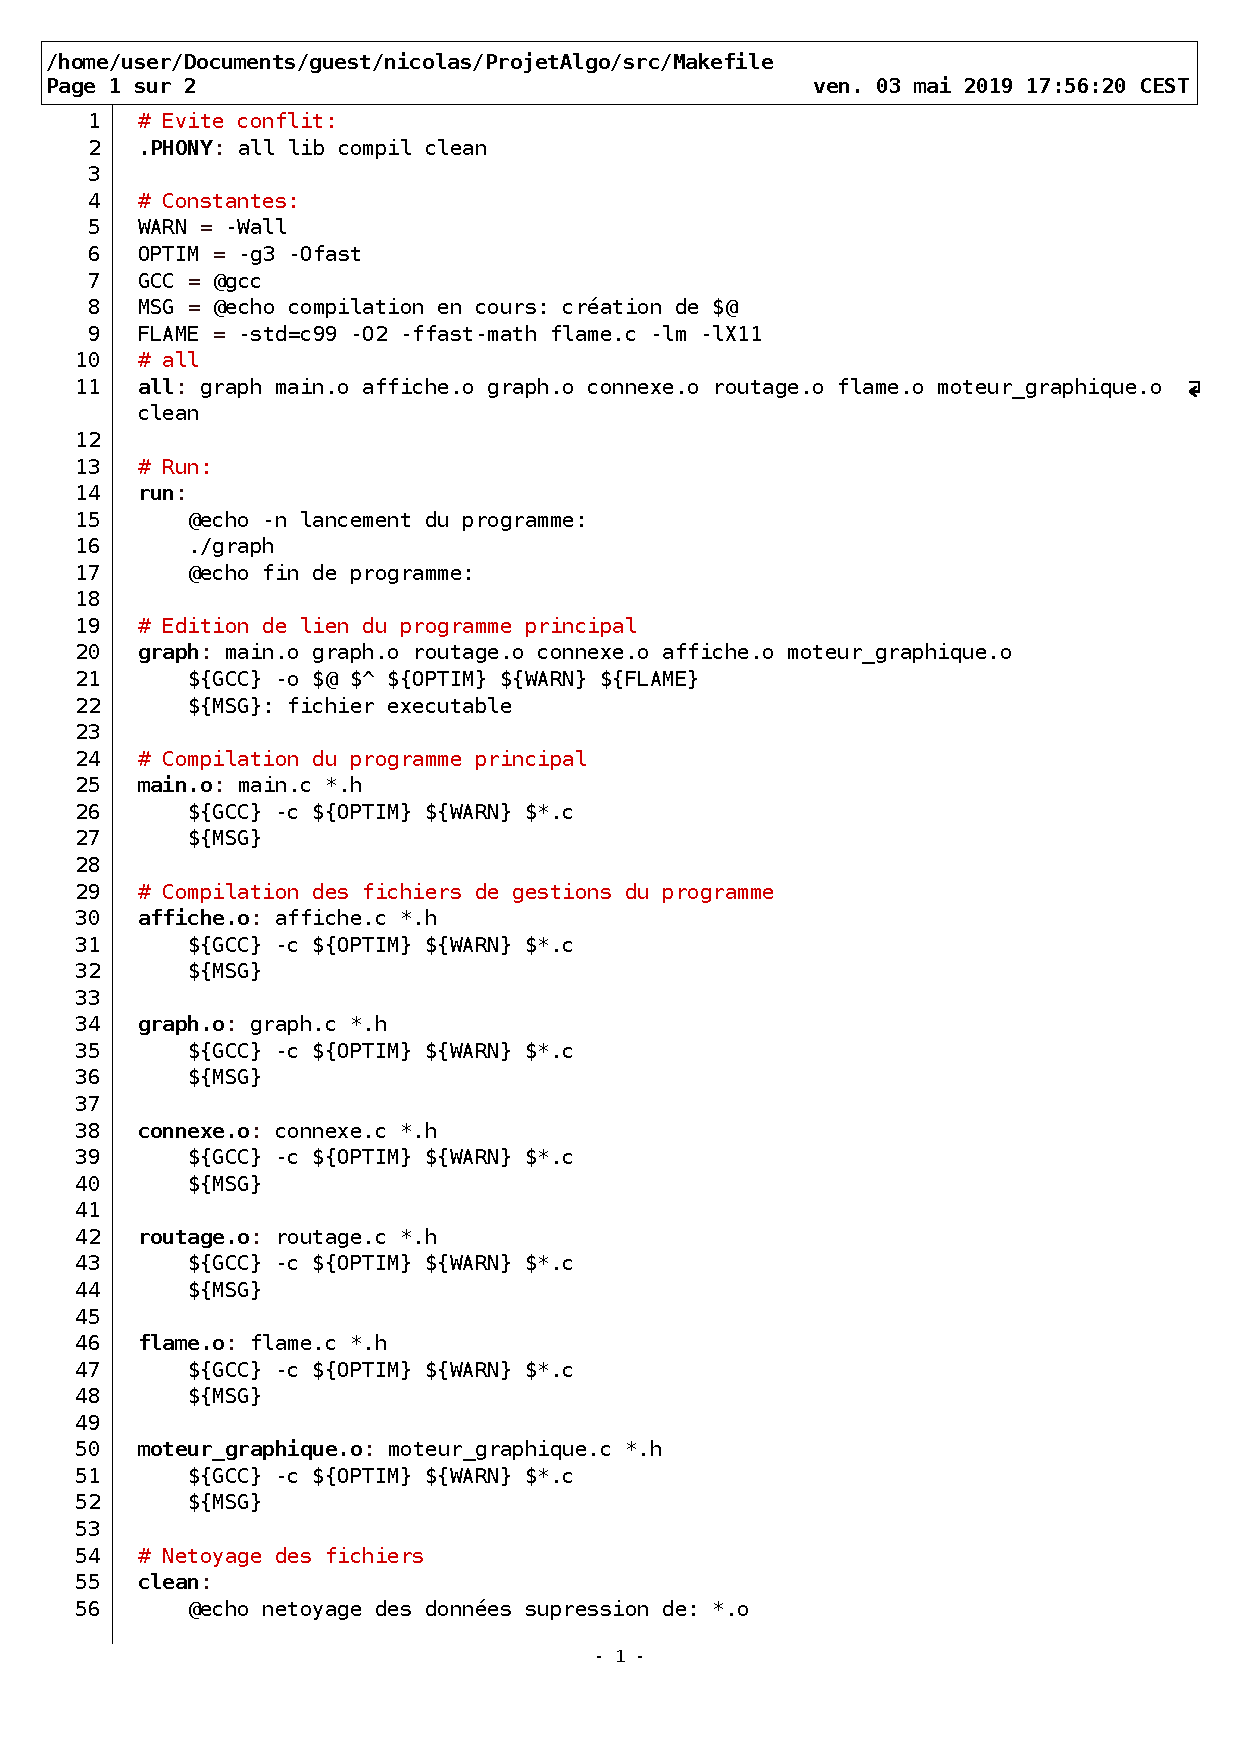
\includepdf[pages=1-2]{Makefile}

\section{Création du graphe}
Fichiers pour la création du graphe:
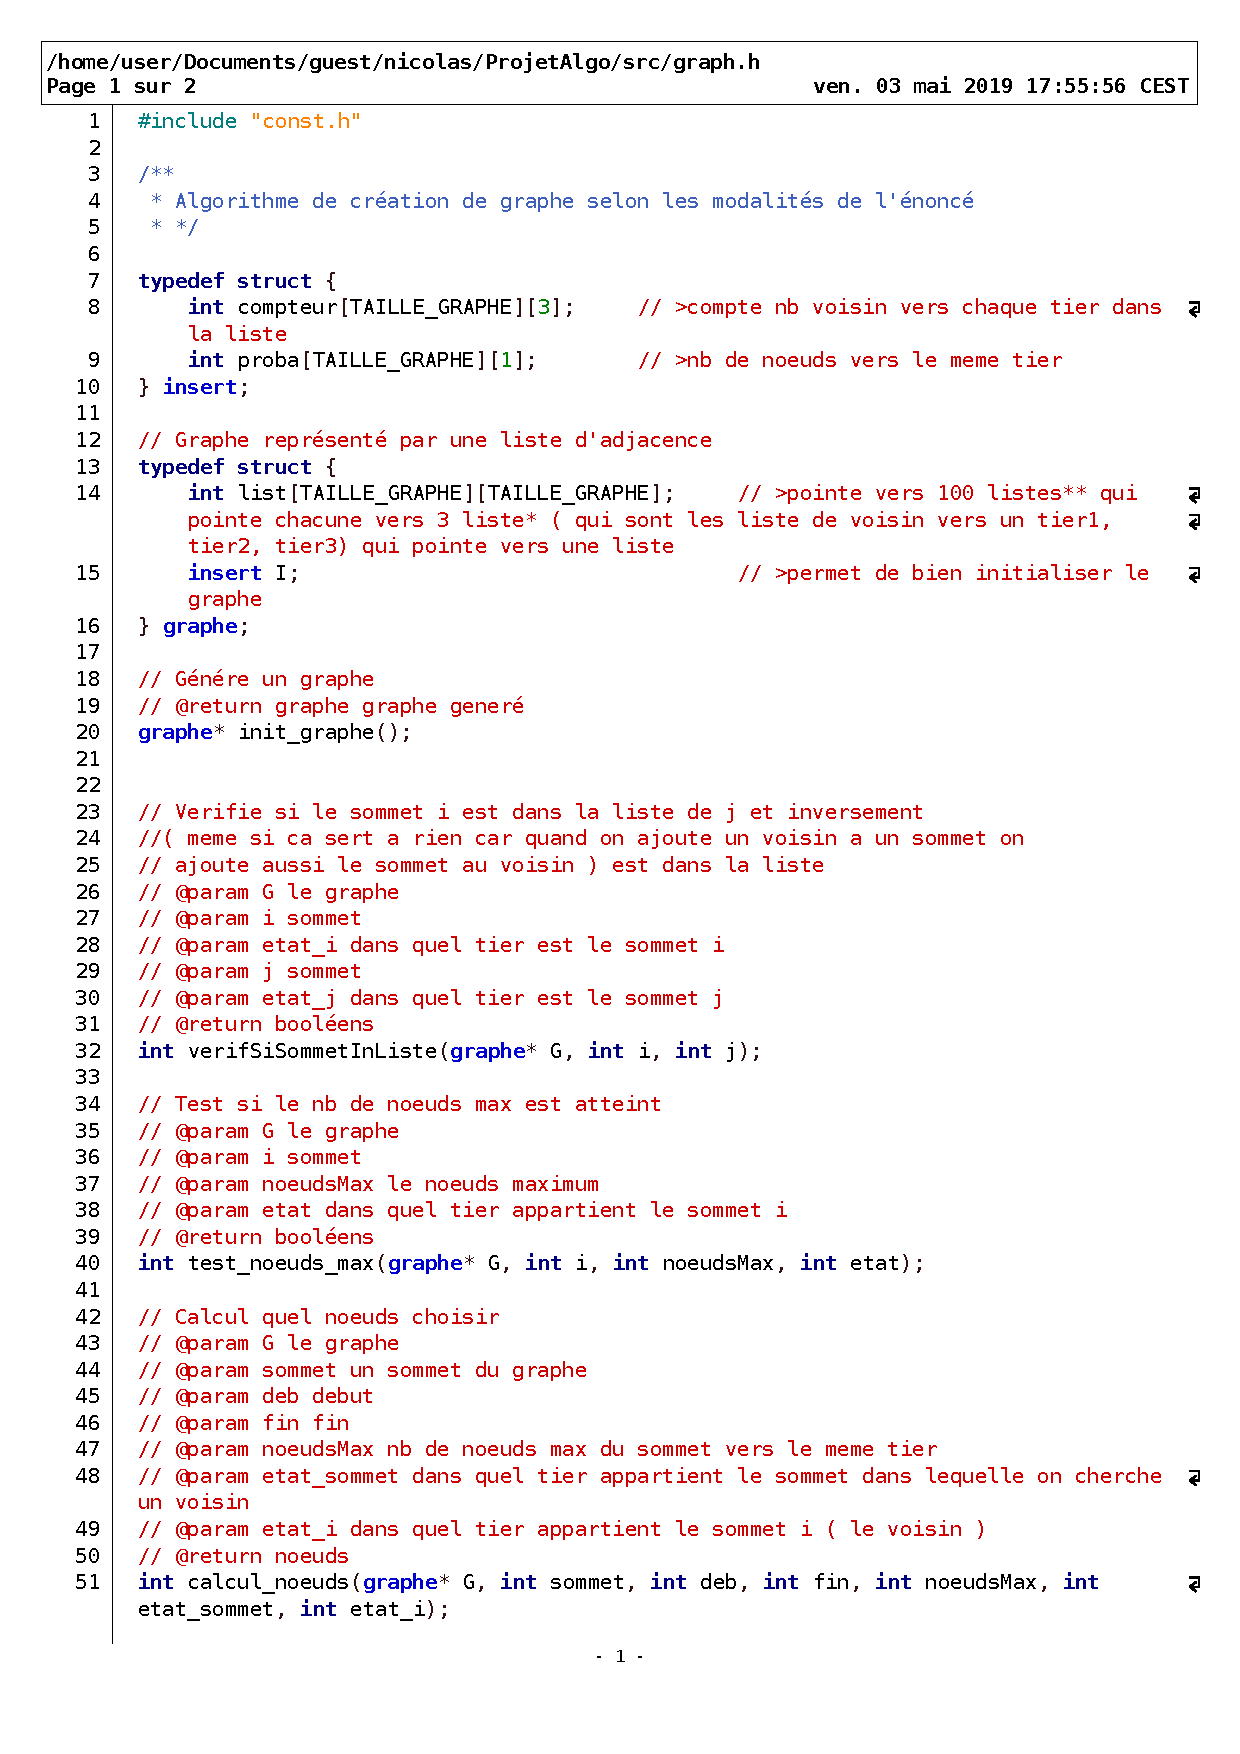
\includepdf[pages=1-2]{graph_h}
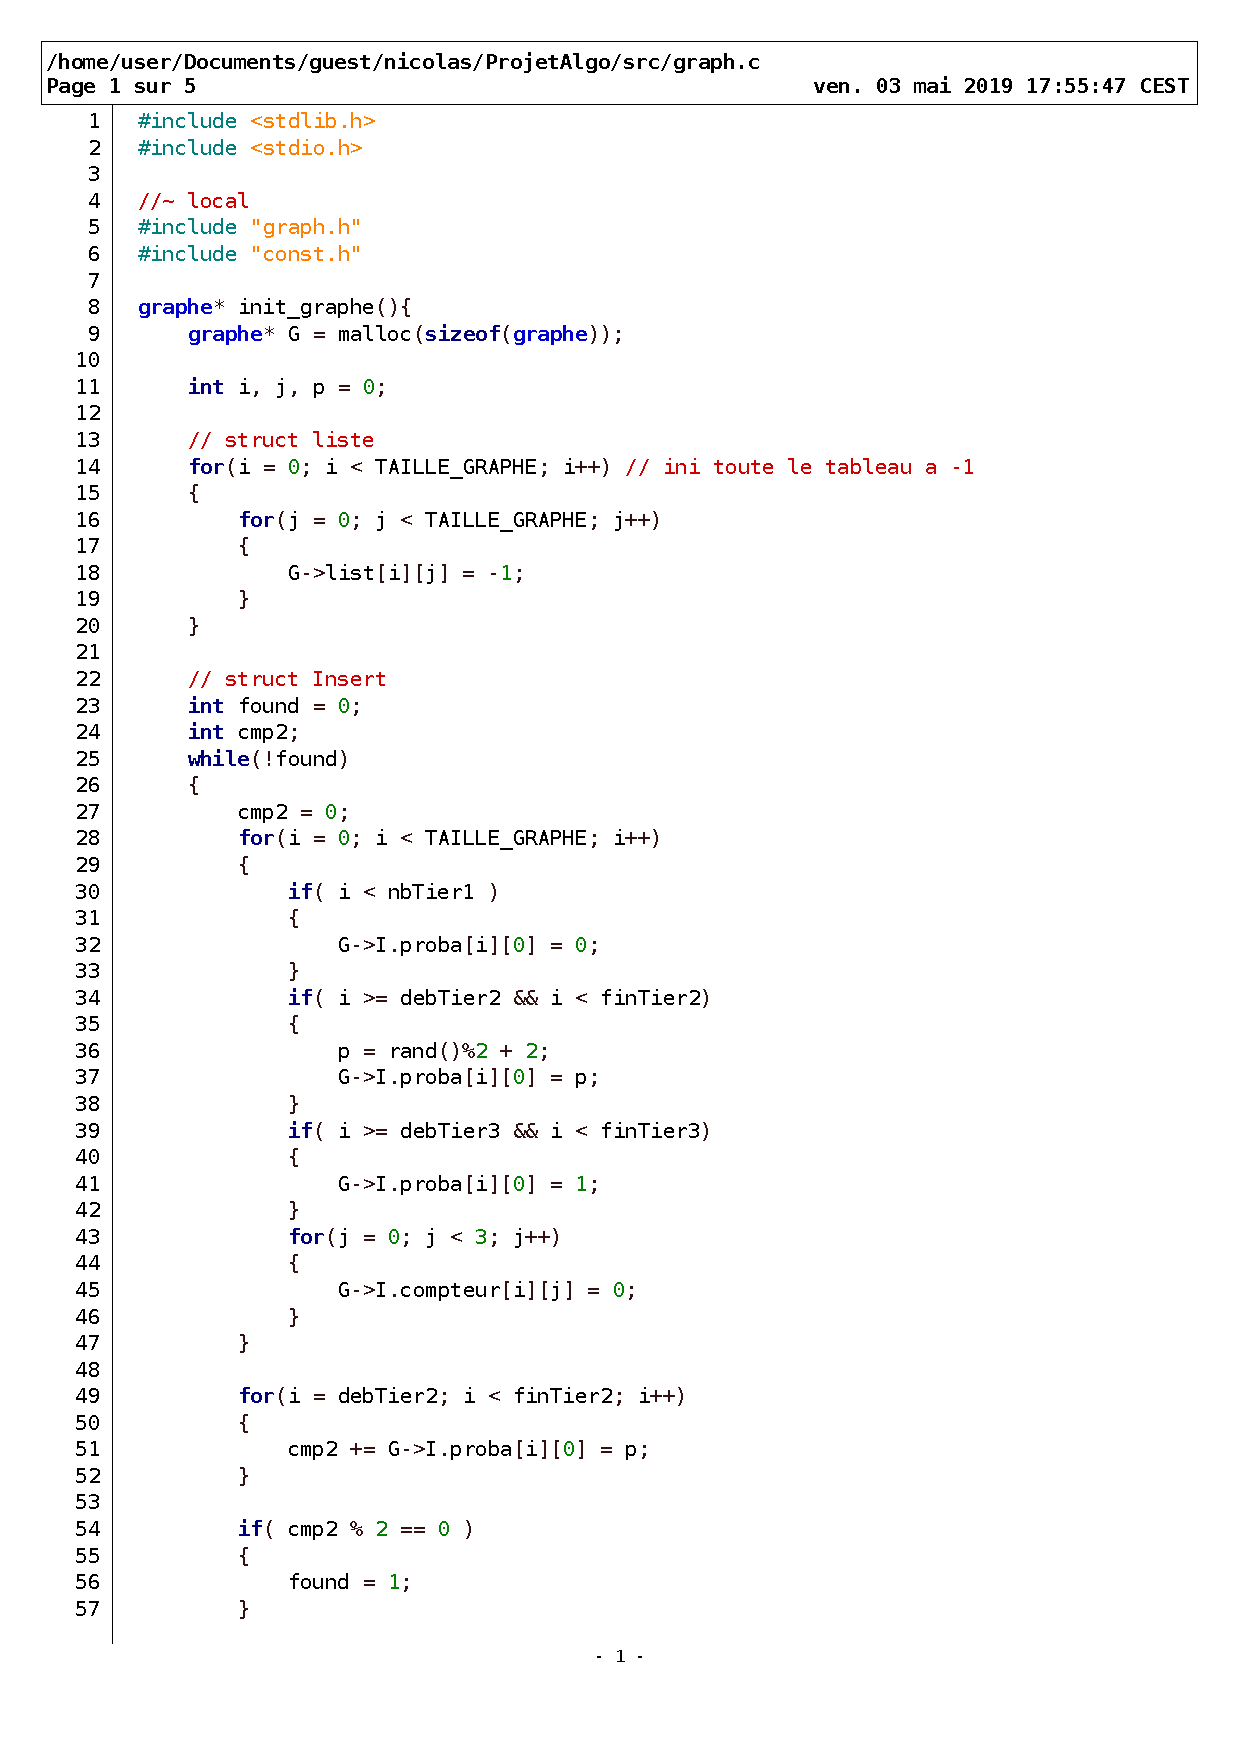
\includepdf[pages=1-5]{graph_c}

\section{Vérification de la connexité}
Fichiers pour vérifier la connexité du graphe:
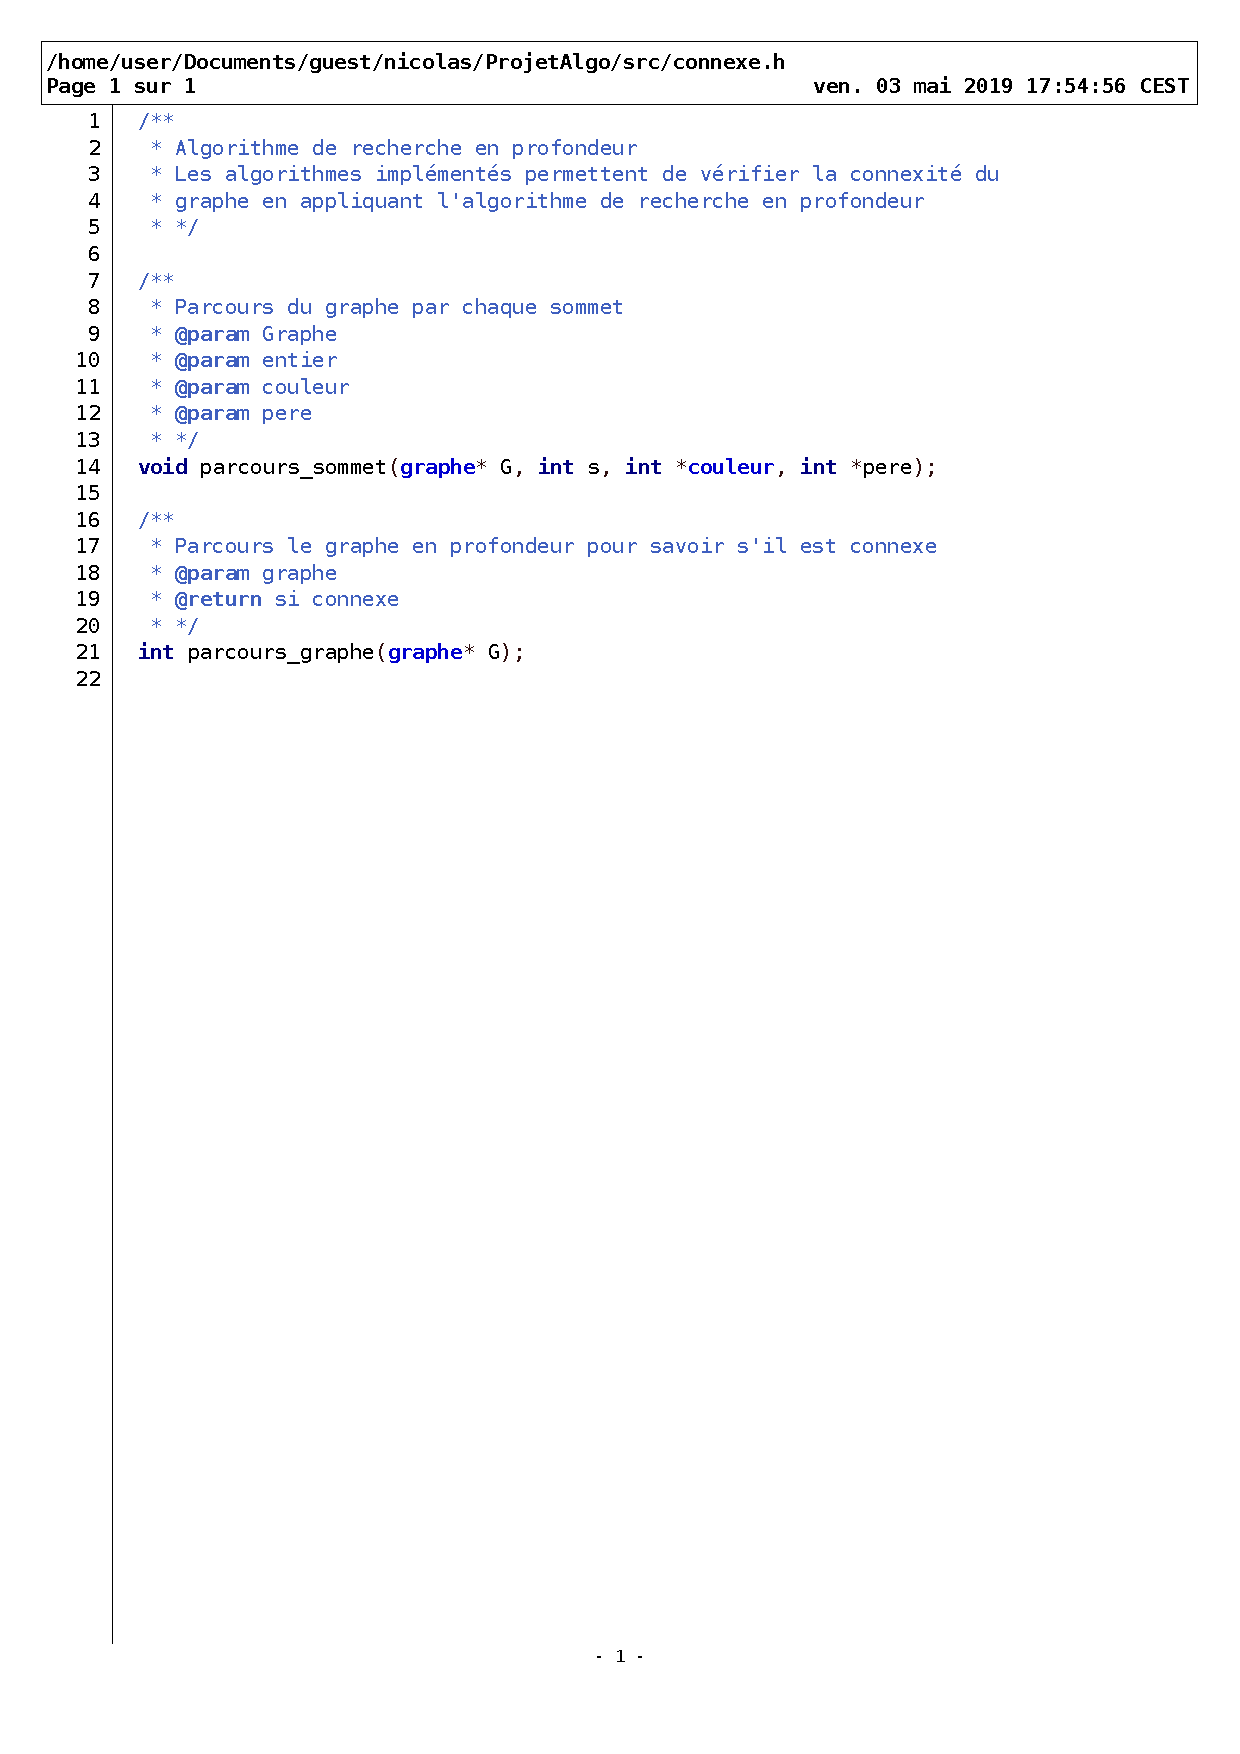
\includepdf{connexe_h}
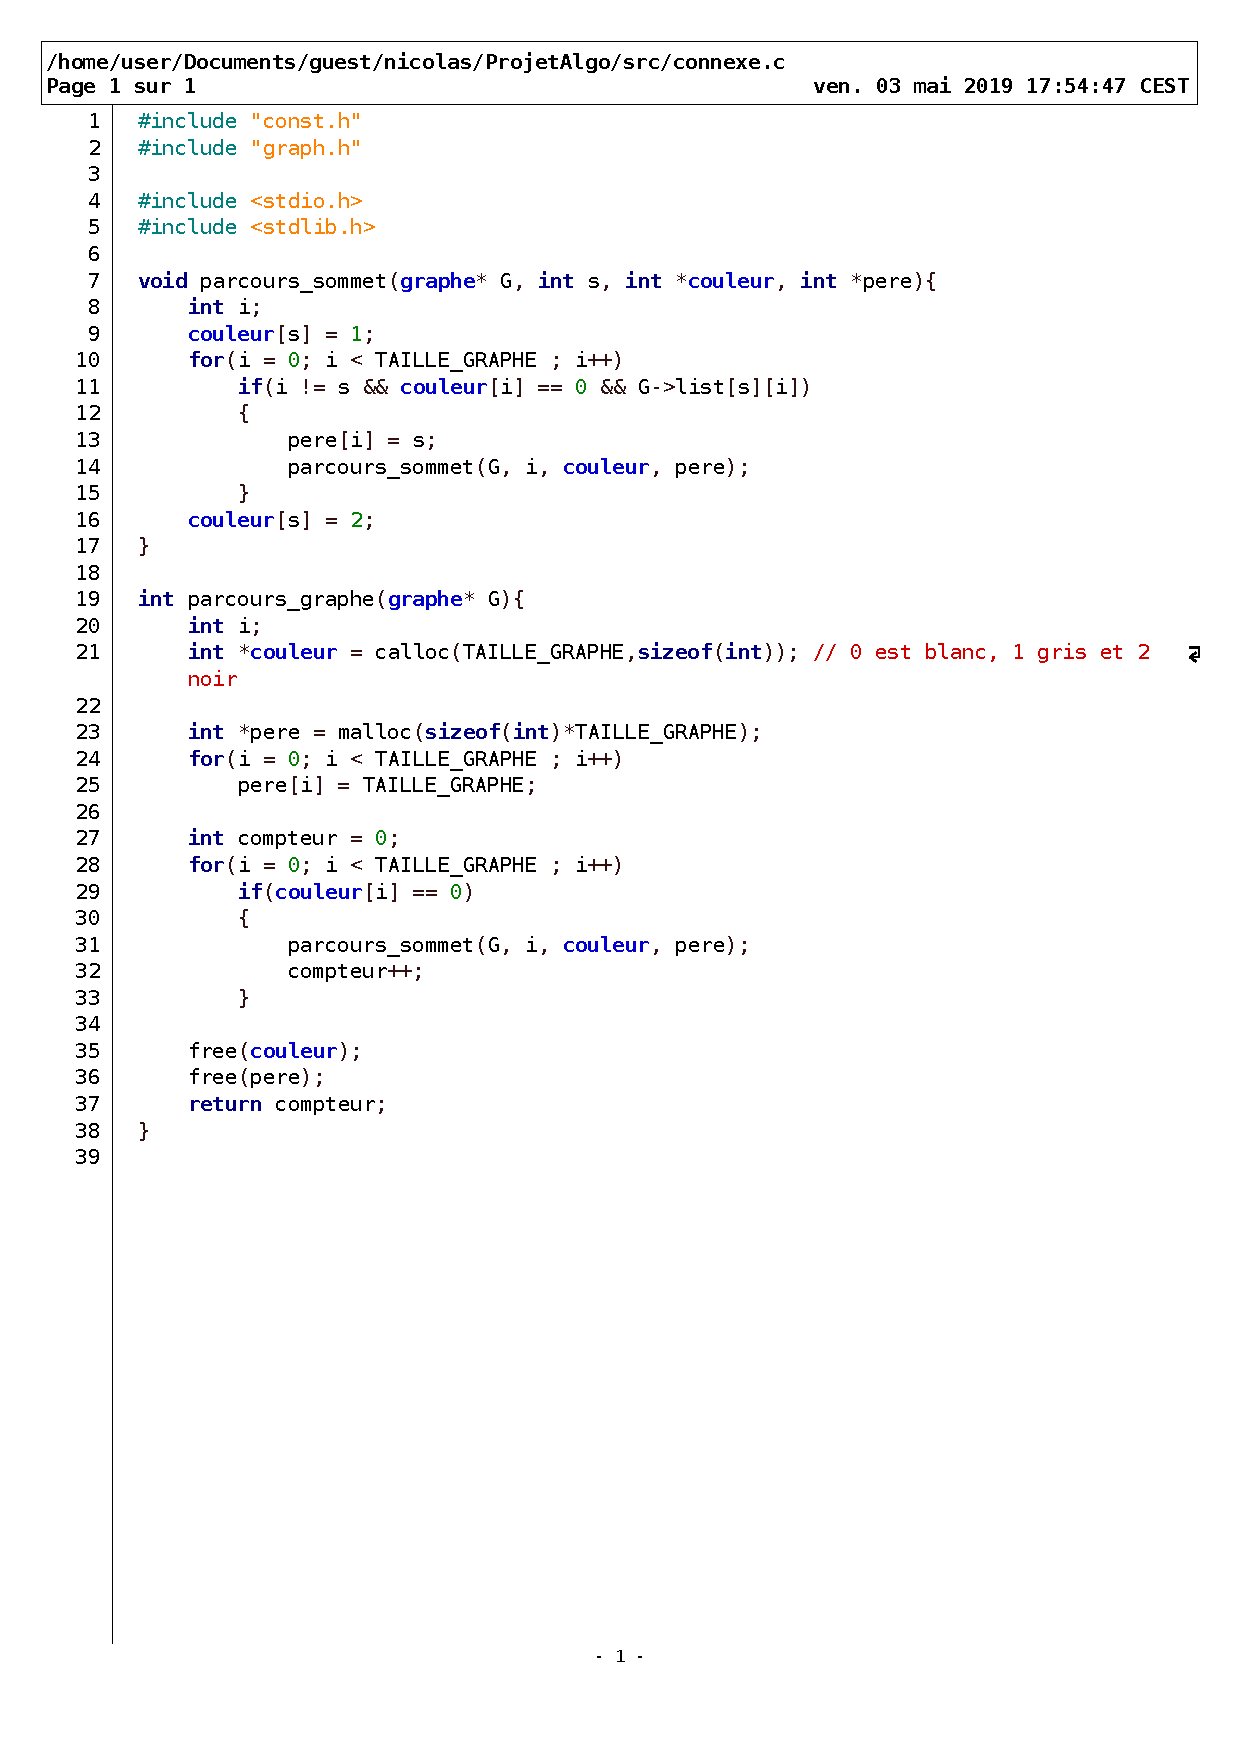
\includepdf{connexe_c}

\section{Création de la table de routage}
Fichiers pour la création de la table de routage:
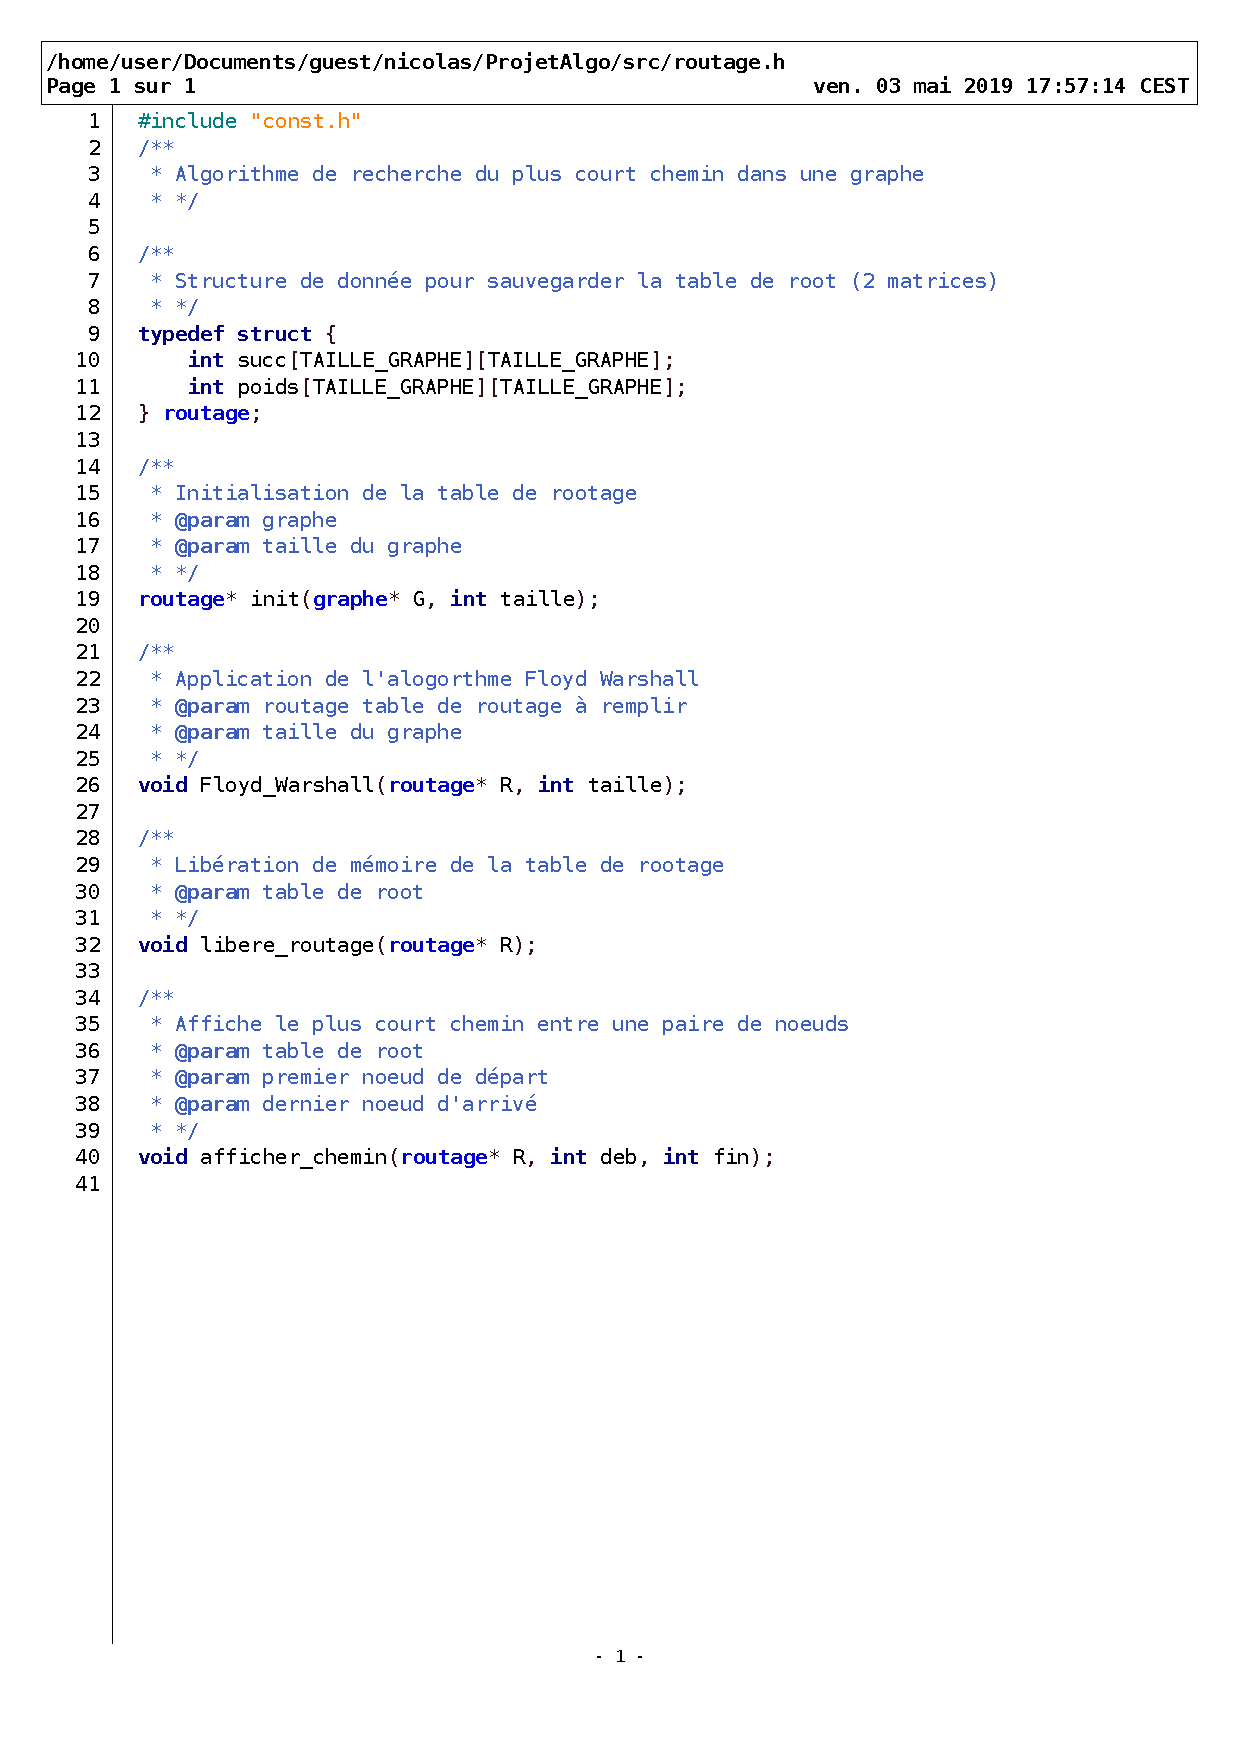
\includepdf{routage_h}
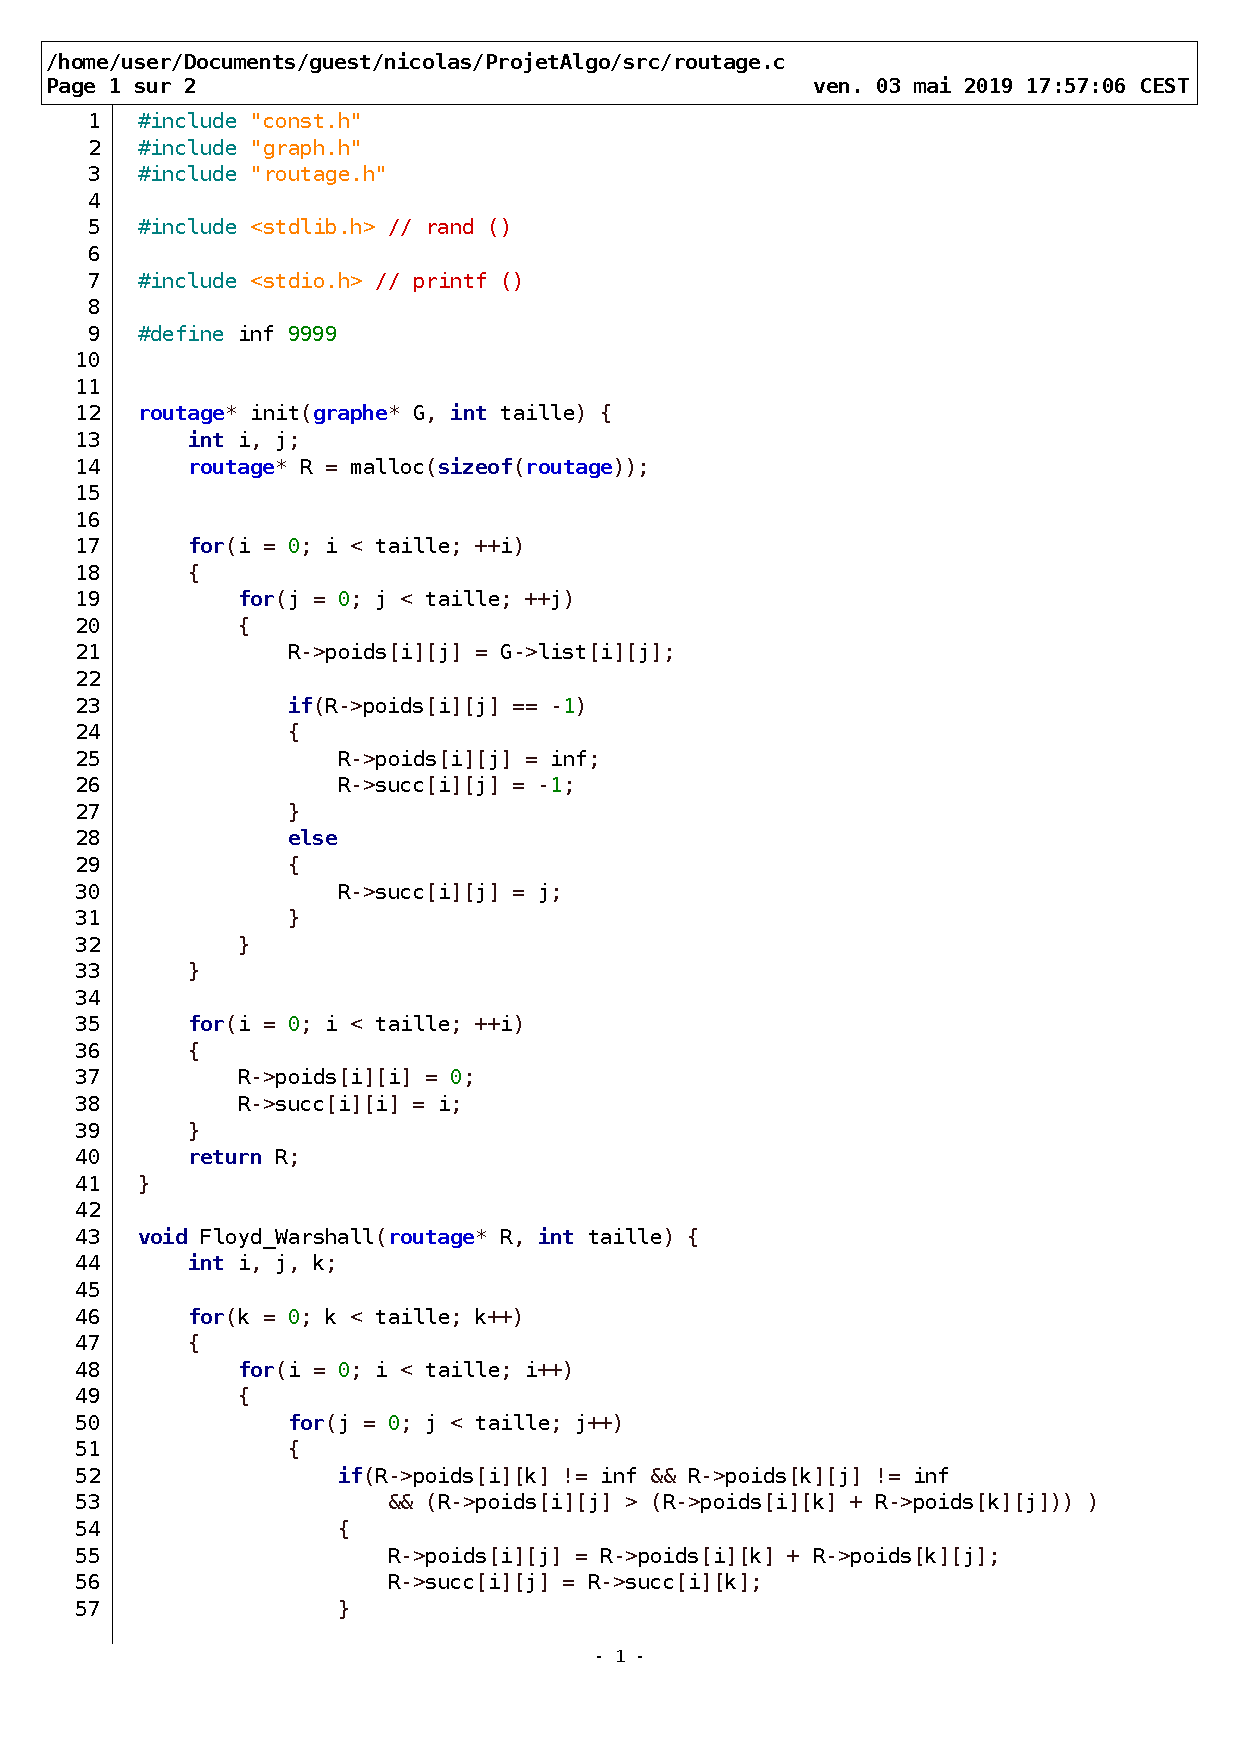
\includepdf[pages=1-2]{routage_c}

\section{Affichage}
Fichiers pour l'affichage graphe:
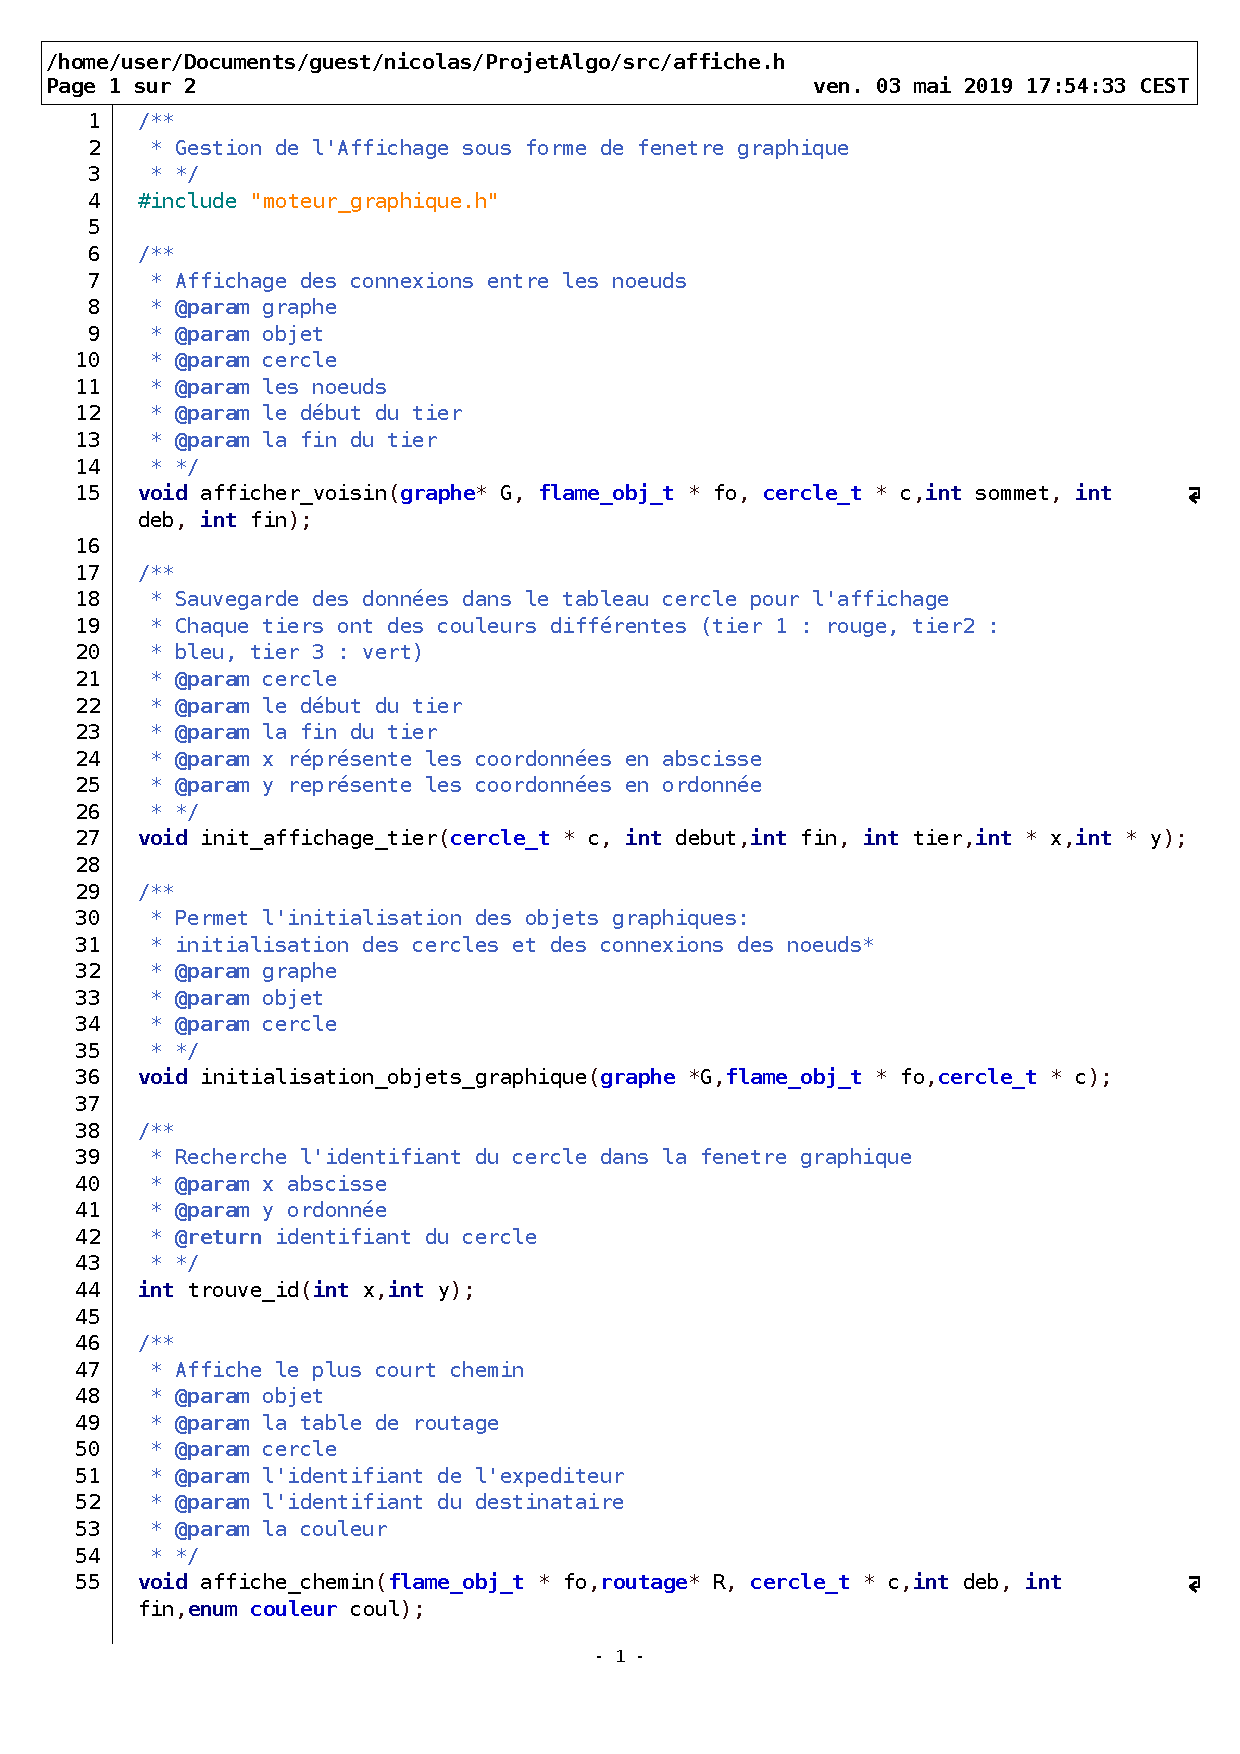
\includepdf[pages=1-2]{afficher_h}
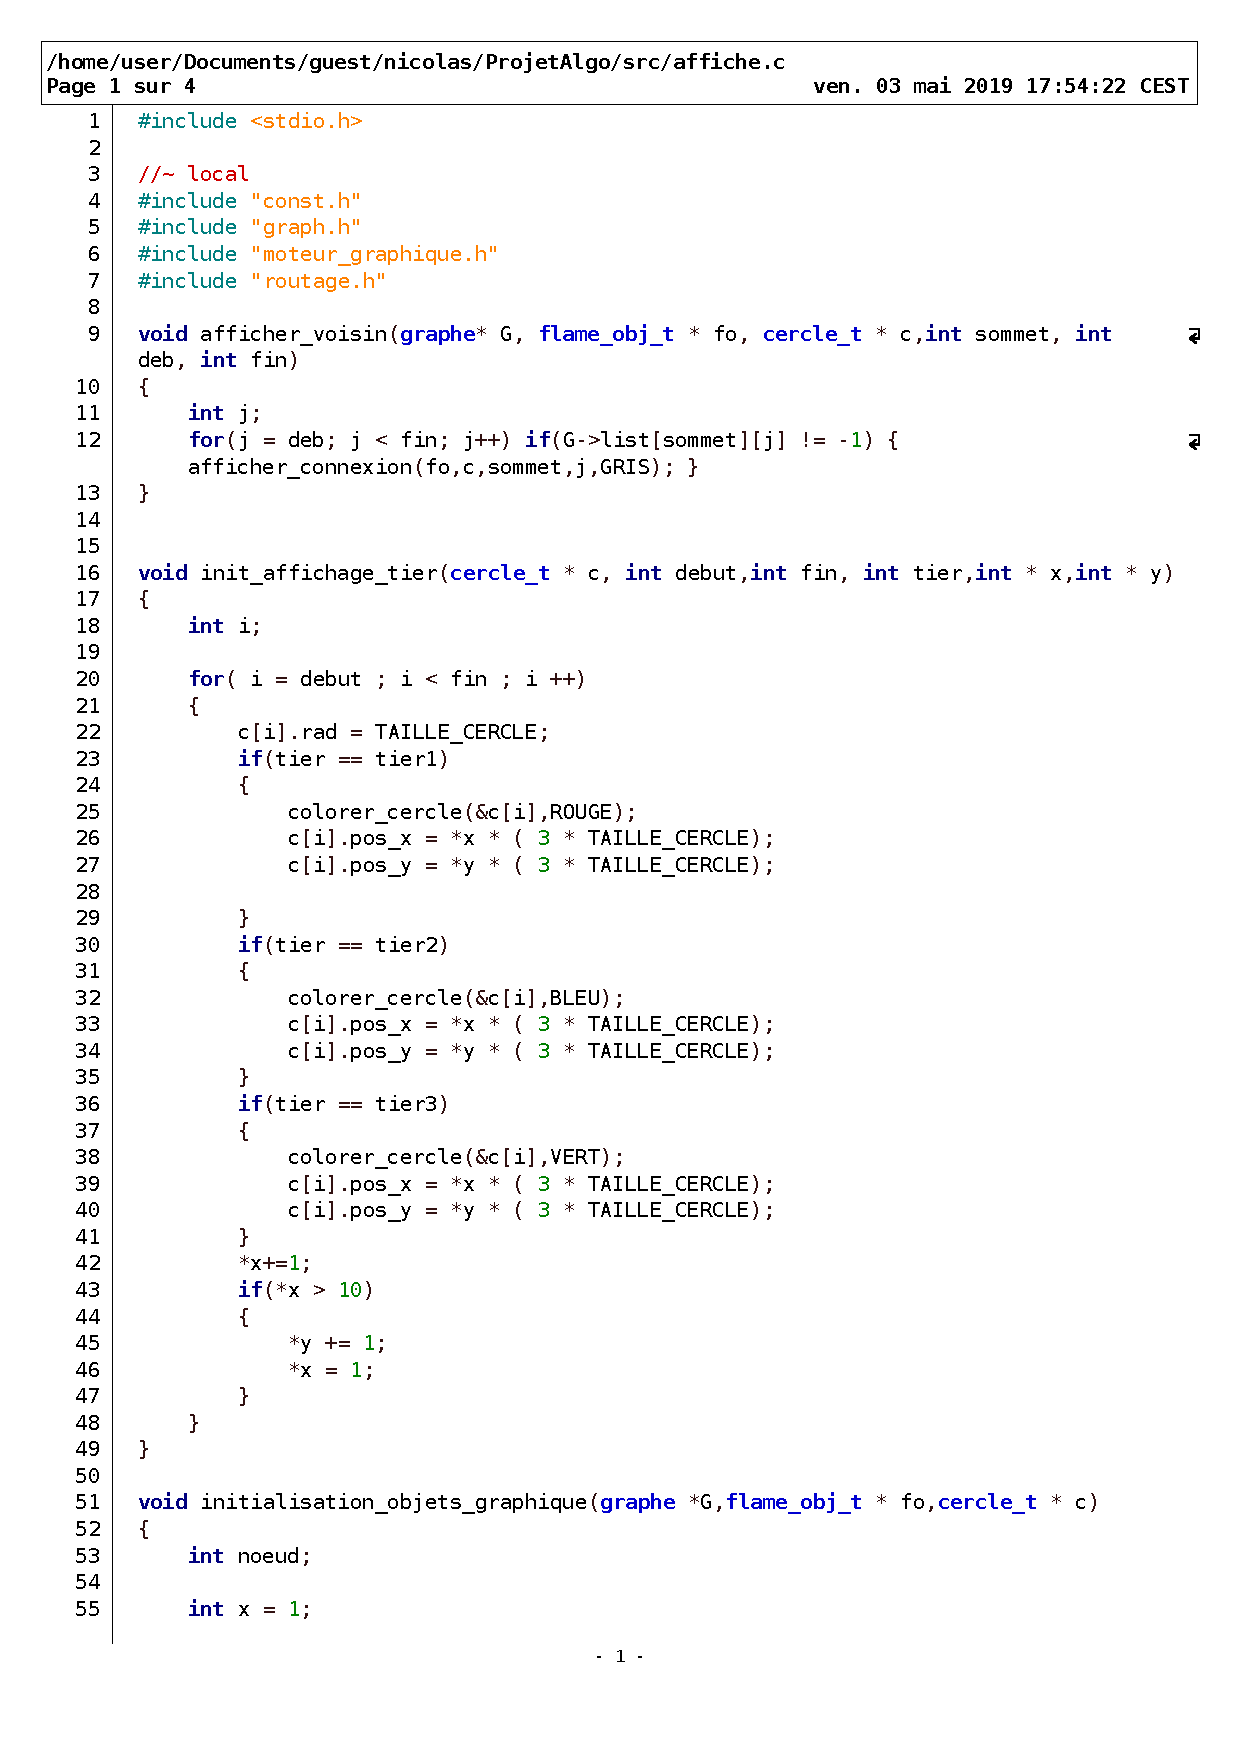
\includepdf[pages=1-4]{afficher_c}
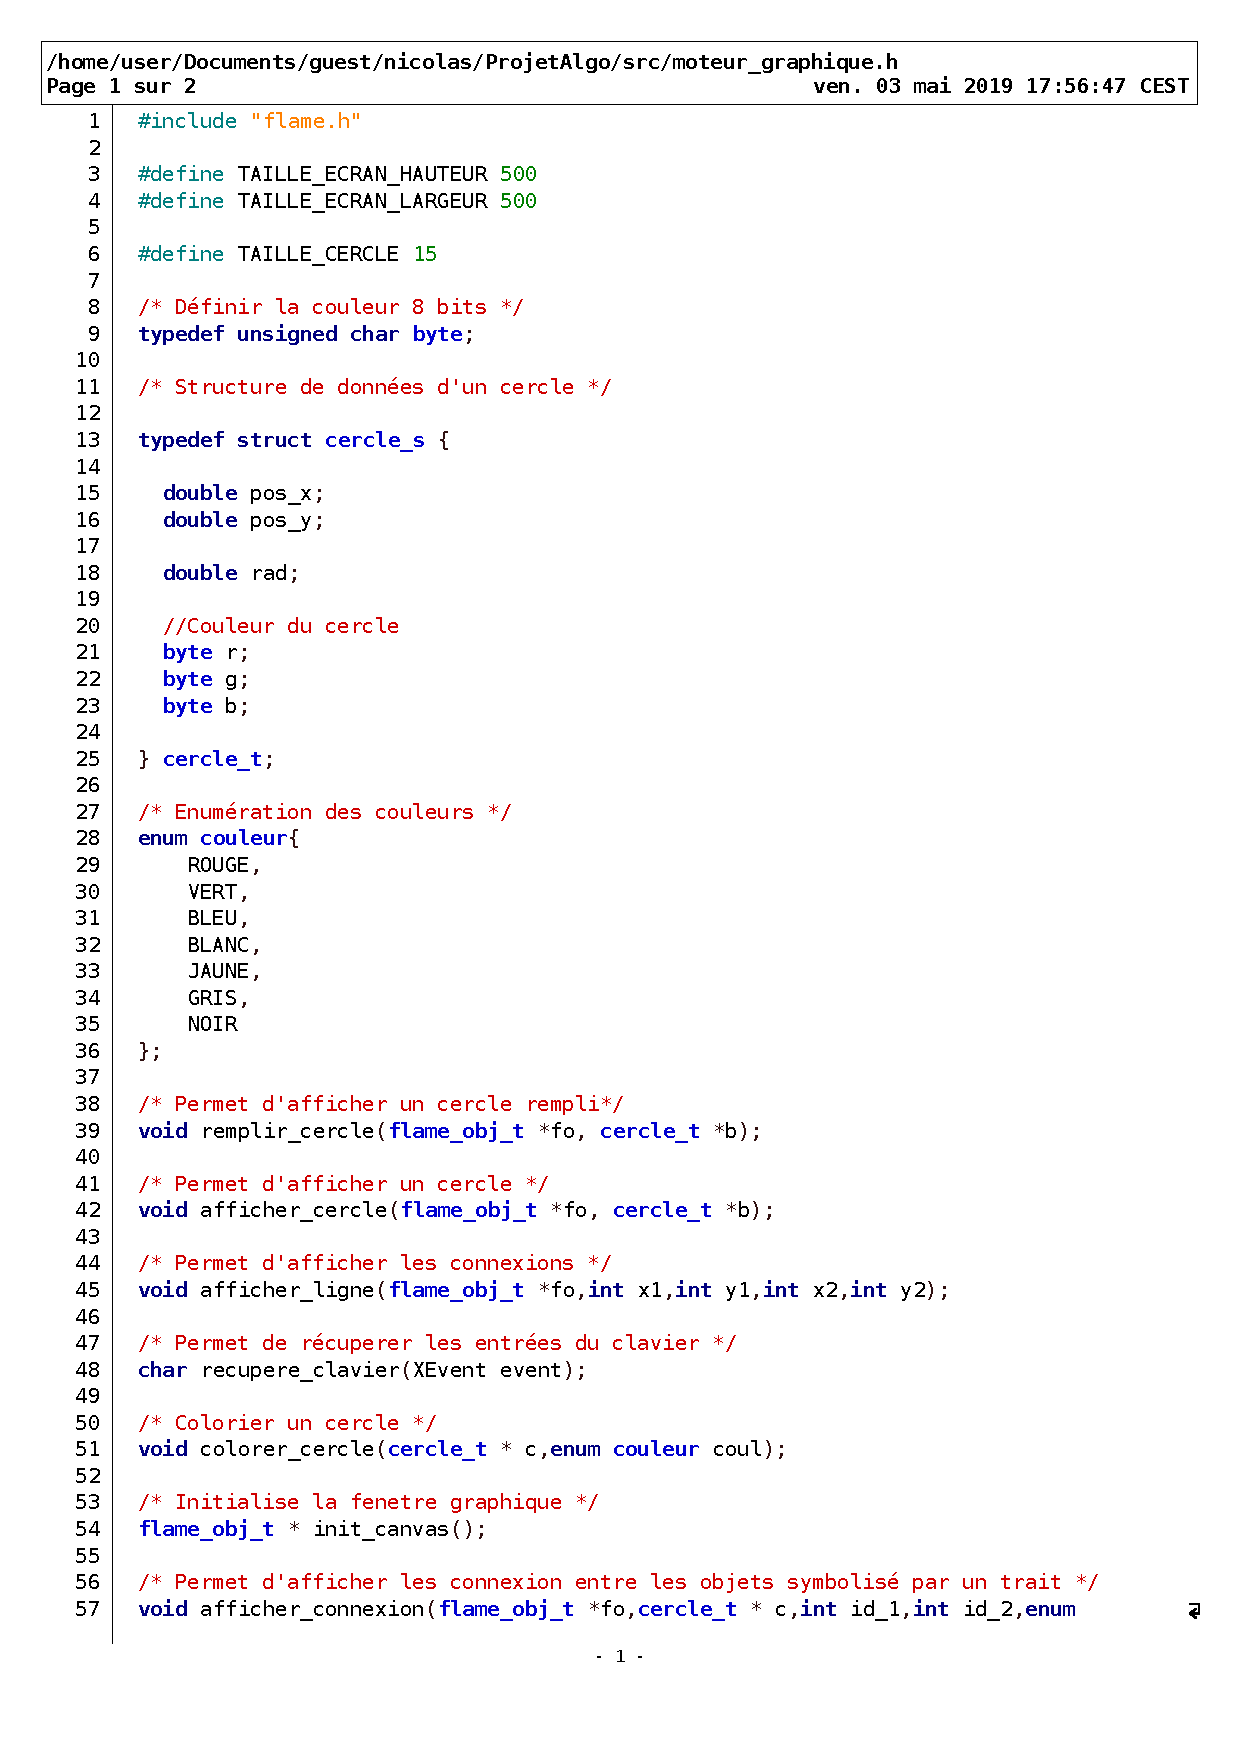
\includepdf[pages=1-2]{moteur_graphique_h}
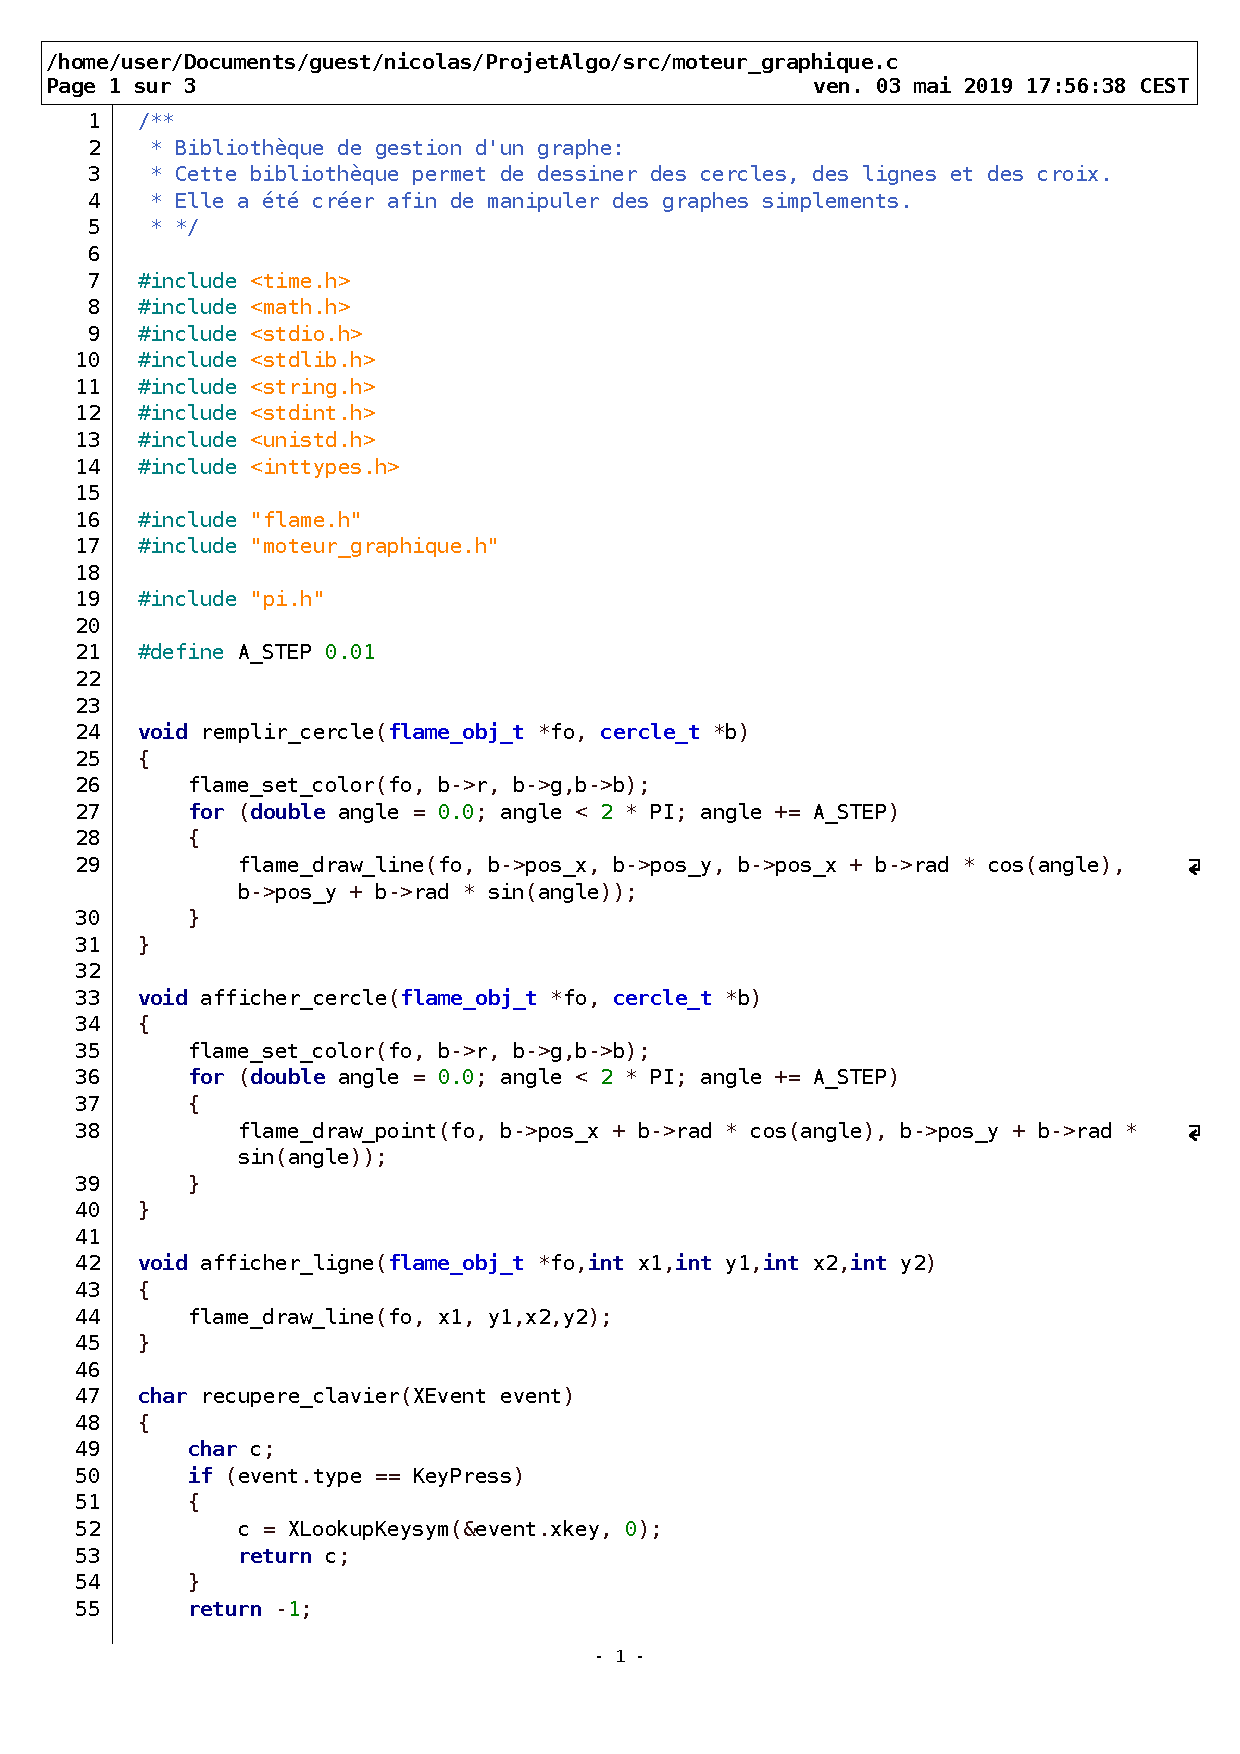
\includepdf[pages=1-3]{moteur_graphique_c}

\section{Les autres fichiers}
\subsection{Constantes}
Fichier pour les définitions des constantes:
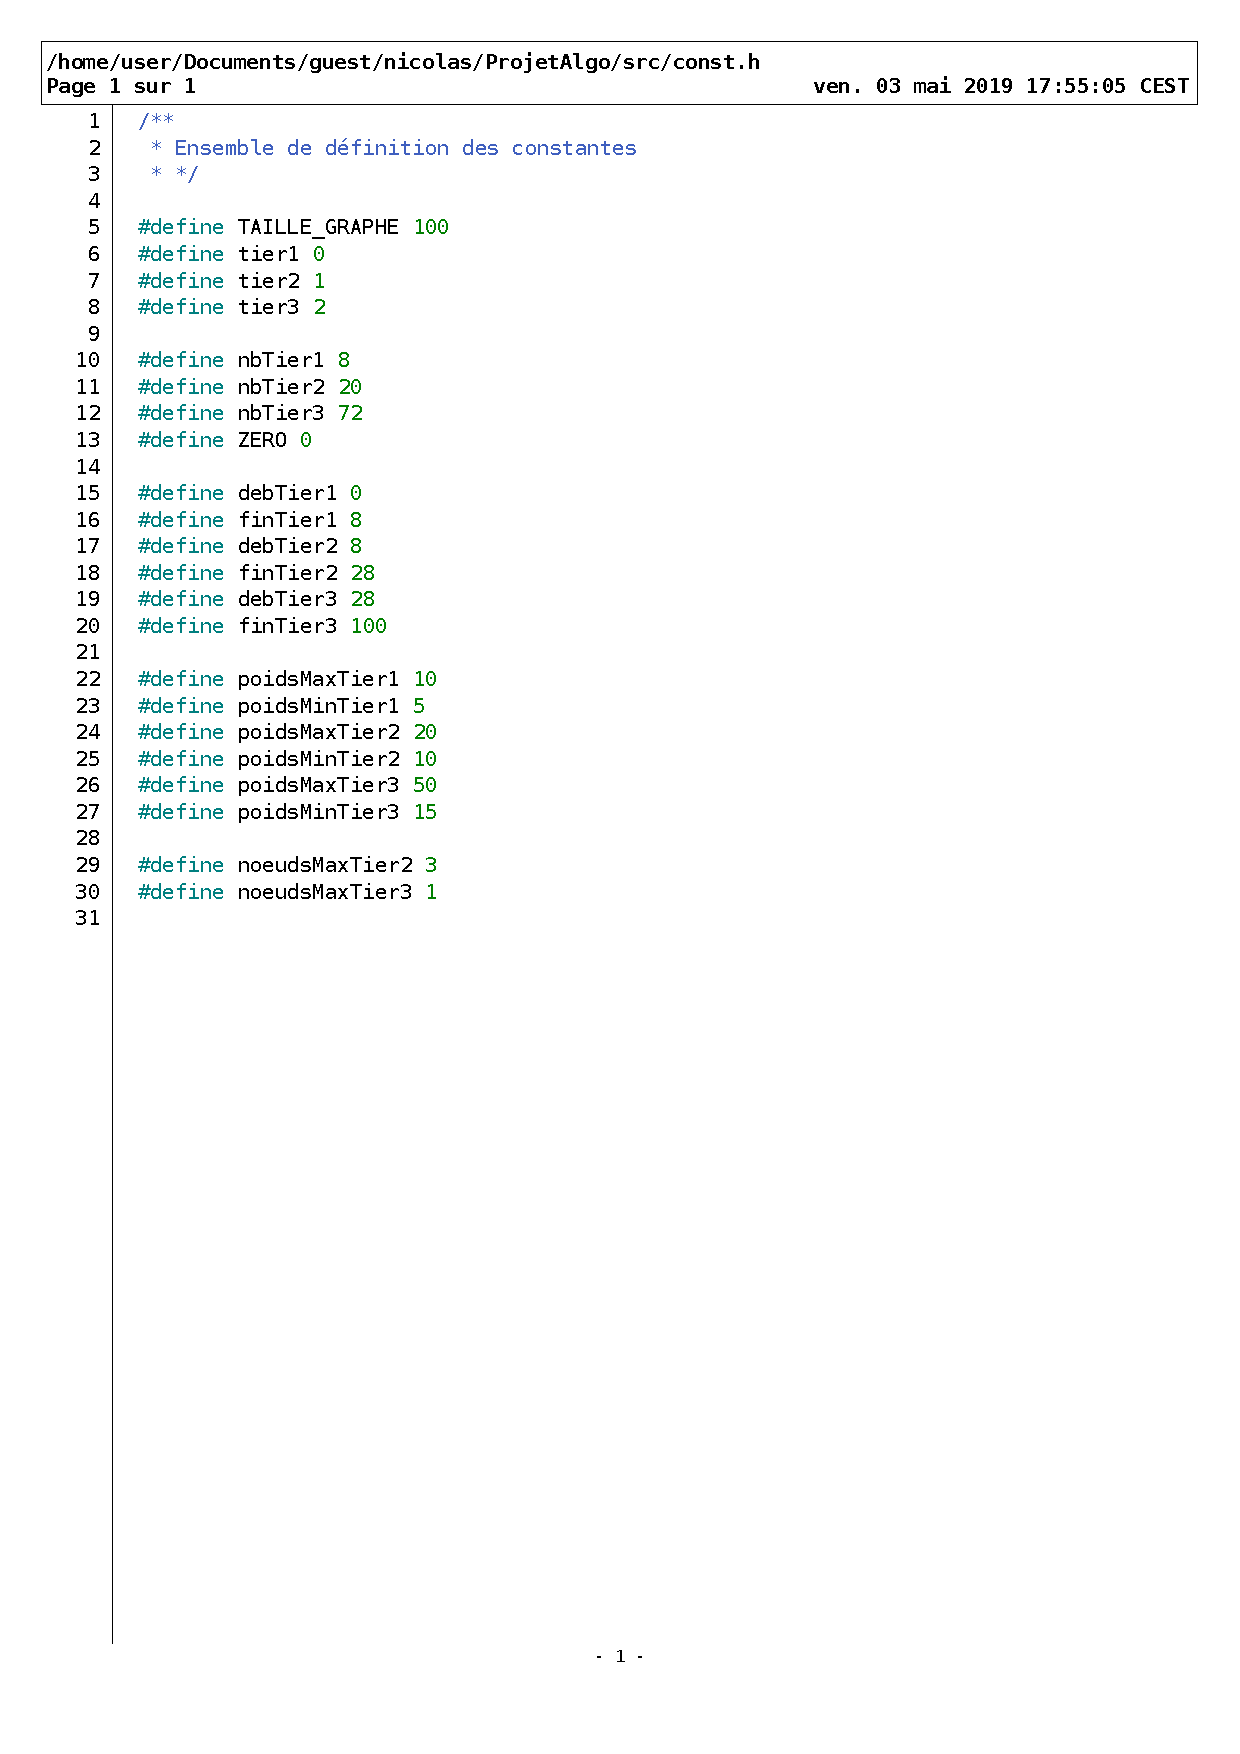
\includepdf{const_h}

\subsection{Bibliothèque flame11}
Code source de la bibliothèque flame11 crée par Yaspr, voici le lien github :
\begin{center}
    \url{https://github.com/yaspr/flame11}    
\end{center}
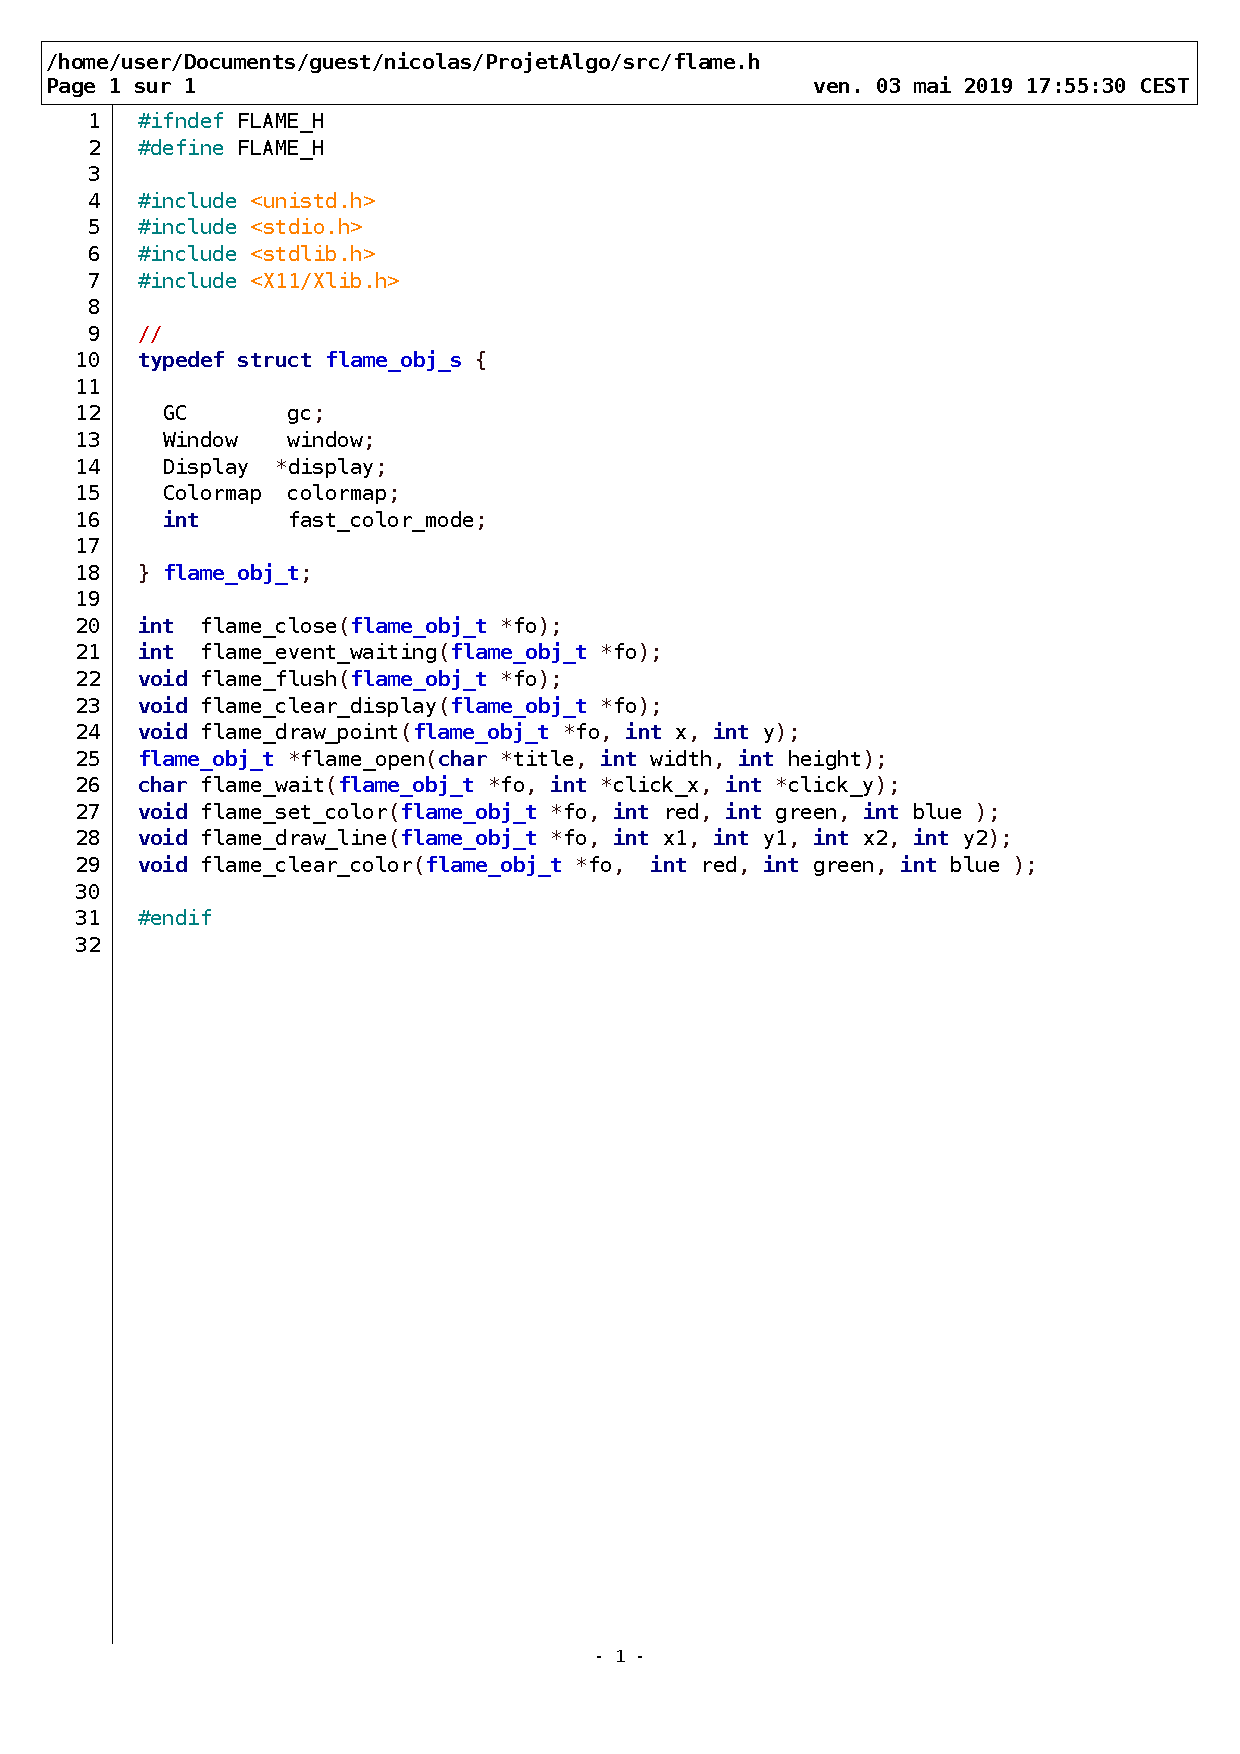
\includepdf{flame_h}
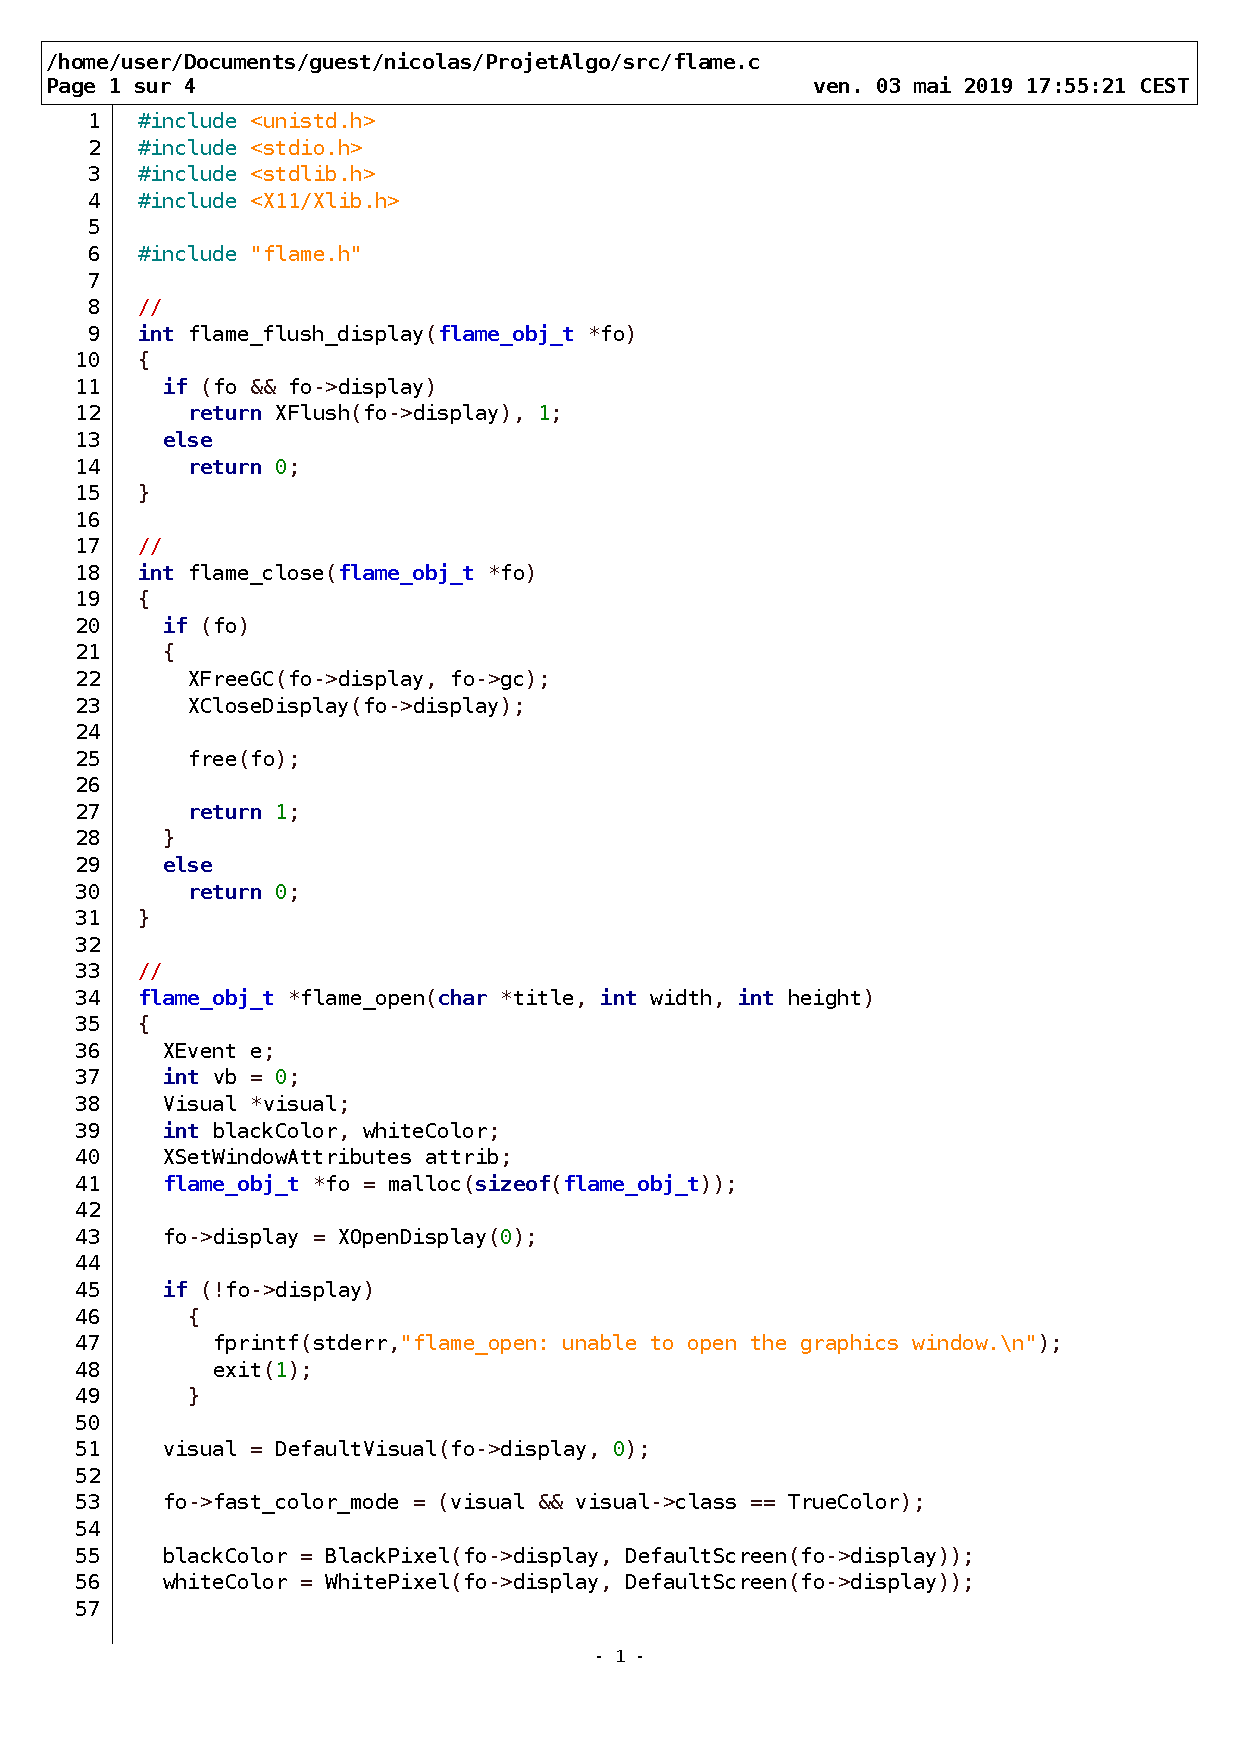
\includepdf[pages=1-4]{flame_c}
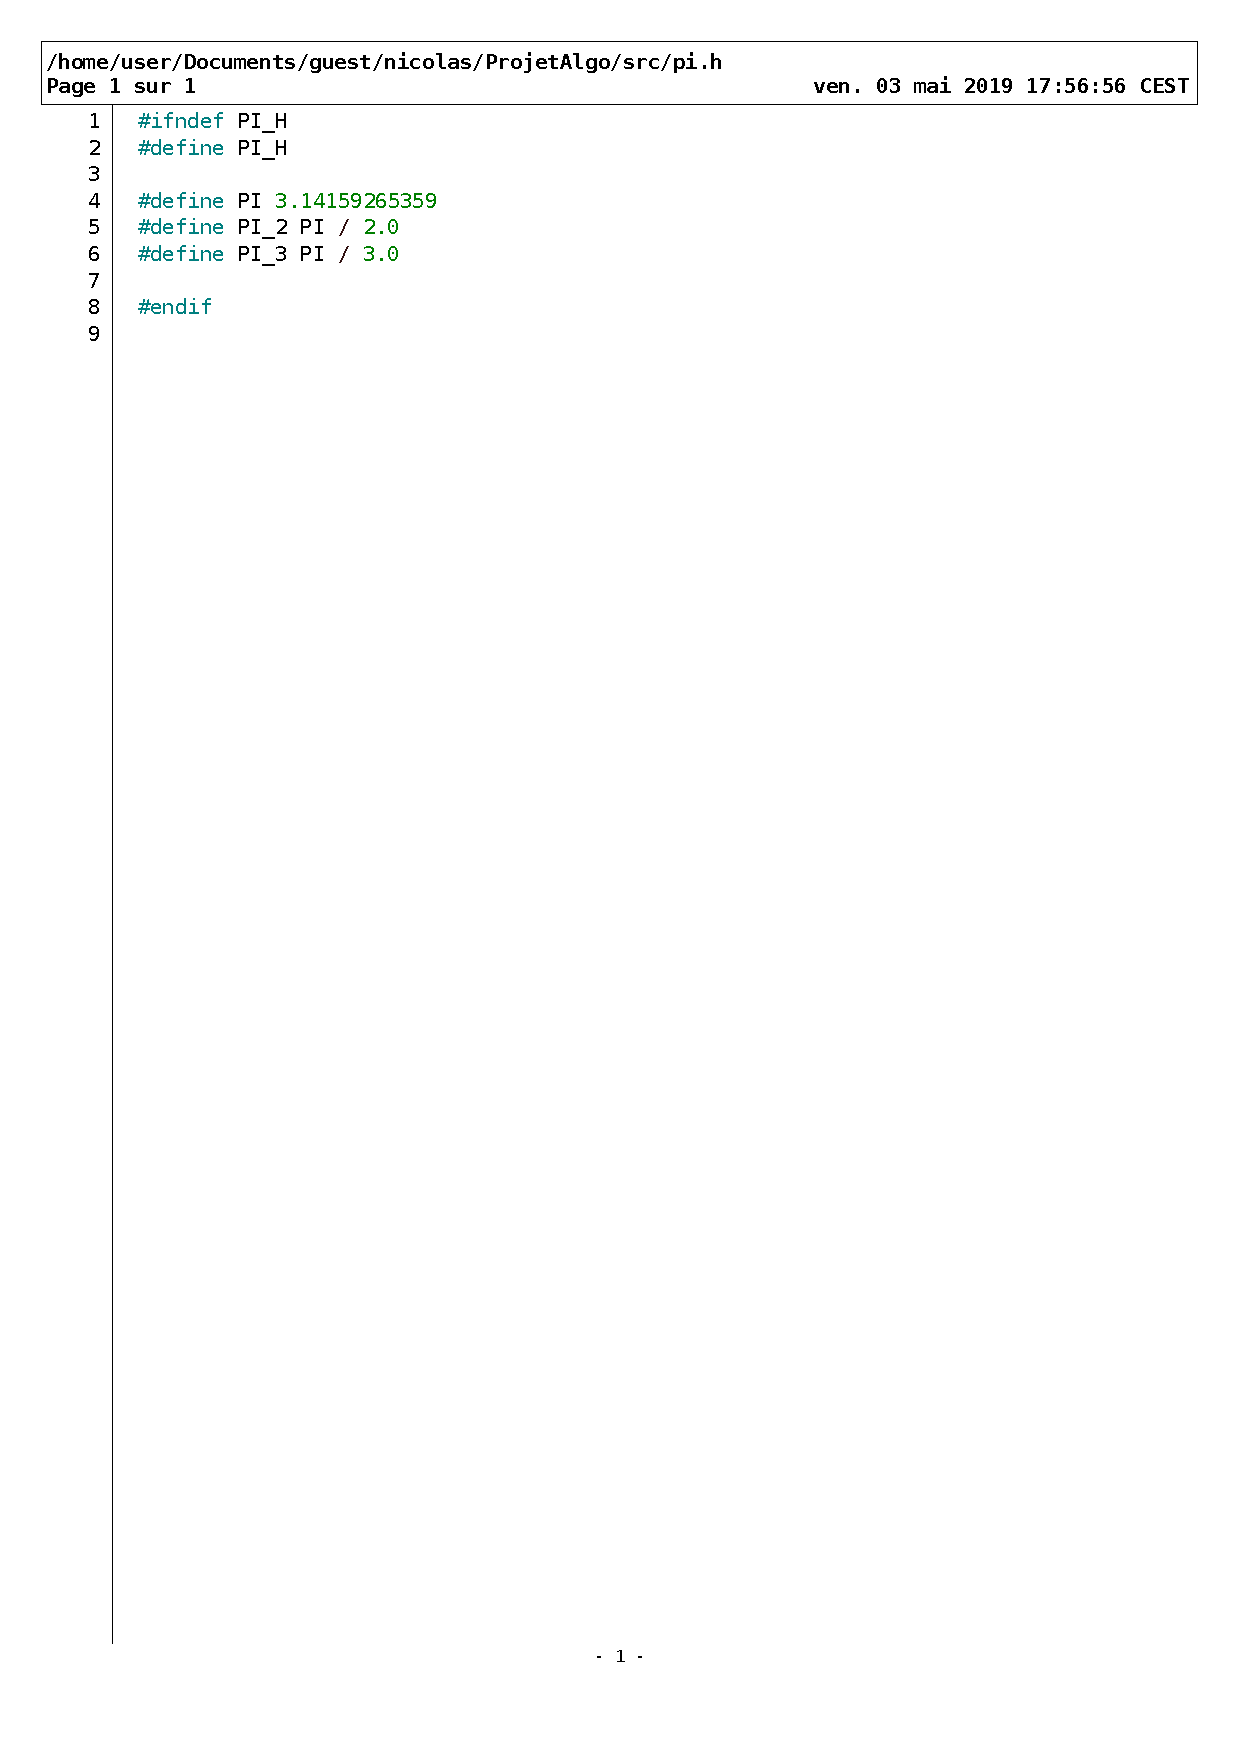
\includepdf{pi_h}

\end{document}